\documentclass{article}
\usepackage{amsmath}
\usepackage{fancyhdr}
\usepackage{amssymb}
\usepackage{amsthm}
\usepackage{graphicx}
\usepackage{varioref}
\usepackage{verbatim} 
\usepackage{multicol}
\usepackage{enumerate}
\usepackage[normalem]{ulem}
%\usepackage[margin=1in]{geometry}
\usepackage{caption}
\usepackage{subcaption}
\usepackage[T1]{fontenc}
\usepackage[margin=1in]{geometry}
\usepackage{thm-restate}
\usepackage{enumitem}
\usepackage{multicol}
\usepackage{float}


\usepackage{mathrsfs}

\usepackage{url}\urlstyle{same}
\usepackage{xspace}
\usepackage{thm-restate}

% Nicer font
\usepackage{mathpazo}


% Microtype
\usepackage{microtype}

% TikZ
\usepackage{tikz}
\usetikzlibrary{calc}
\usetikzlibrary{decorations.pathmorphing}
\usetikzlibrary{decorations.markings}

% Support eps figures
\usepackage{epstopdf}

% Hypertext package
\usepackage[colorlinks = true]{hyperref}
% Title and authors
%\hypersetup{
%  pdftitle = {},
%  pdfauthor = {}
%}
% Color definitions
\usepackage{xcolor}
\definecolor{darkred}  {rgb}{0.5,0,0}
\definecolor{darkblue} {rgb}{0,0,0.5}
\definecolor{darkgreen}{rgb}{0,0.5,0}
% Color links
\hypersetup{
  urlcolor   = blue,         % color of external links
  linkcolor  = darkblue,     % color of internal links
  citecolor  = darkgreen,    % color of links to bibliography
  filecolor  = darkred       % color of file links
}

% Clever references
\usepackage{cleveref}%[nameinlink]
\crefname{lemma}{Lemma}{Lemmas}
\crefname{proposition}{Proposition}{Propositions}
\crefname{definition}{Definition}{Definitions}
\crefname{theorem}{Theorem}{Theorems}
\crefname{conjecture}{Conjecture}{Conjectures}
\crefname{corollary}{Corollary}{Corollaries}
\crefname{section}{Section}{Sections}
%\crefname{property}{Property}{Properties}
\crefname{appendix}{Appendix}{Appendices}
\crefname{figure}{Fig.}{Figs.}
\crefname{equation}{Eq.}{Eqs.}
\crefname{table}{Table}{Tables}
\crefname{claim}{Claim}{Claims}
%\crefname{item}{Property}{Properties}

%%%%%%%%%%%%%%%%%%%%%%%%%
%  N E W T H E O R E M  %
%%%%%%%%%%%%%%%%%%%%%%%%%

\newtheorem{theorem}{Theorem}
\newtheorem{lemma}[theorem]{Lemma}
\newtheorem{proposition}[theorem]{Proposition}
\newtheorem{definition}[theorem]{Definition}
\newtheorem{corollary}[theorem]{Corollary}
\newtheorem{conjecture}[theorem]{Conjecture}
\newtheorem{property}[theorem]{Property}
\newtheorem*{conjecture*}{Conjecture}
\newtheorem*{problem}{Problem}
\newtheorem{claim}[theorem]{Claim}
\theoremstyle{definition}
\newtheorem*{remark}{Remark}
\newtheorem*{example}{Example}

\DeclareMathOperator{\E}{\mathrm{E}}		     % expected value
\DeclareMathOperator{\p}{\mathrm{P}}		     % probability

\begin{document}


%+Title
\title{Applications of Graph Theory and Probability in the Board Game \it{Ticket to Ride}}

\author{R. Teal Witter \& Alex Lyford}

\date{\today}
%\date{\today}

\maketitle
%-Title

\begin{multicols}{2}
\section{Introduction}
\subsection{Background}
People have been playing mathematical games
since as early as 2000 B.C.
\cite{cornelius1986historical}.
All along,
players have attempted to devise optimal
strategies, simulate future moves, or identify
flaws that can be exploited.
Mathematics can serve as a particularly powerful tool for
such analysis.
Abbott and Richey used Markov Chains
to find the long term 
distribution of turns players spend in different
properties in the board game
\textit{Monopoly} \cite{abbott1997take, magie1935}.
(They also found that the optimal strategy is to avoid making
moves altogether and instead maximize time spent in jail.)
Lyford et al. investigated the probability and expected value 
in the board game \textit{Camel Up}
\cite{bogen2014, lyford2019using}.
Witter and Lyford generated an optimal winning strategy for the 
board game \textit{Codenames} using matrix rotations
and a combinatorial argument \cite{chvatil2015}.
% TO DO: CITE CODENAMES PAPER IF ACCEPTED

Another example of a game with mathematical underpinnings is
the board game \textit{Ticket to Ride} \cite{moon2004ticket}. 
Players race to connect 
cities and build railroads on a map of the U.S.
Mathematically, the board
can be thought of as a graph where
cities represent vertices and the
routes between them represent edges.
The educational implications of \textit{Ticket to Ride}
have been extensively studied.
Lim applied the game to teach basic graph theory
\cite{lim2007taking}.
Chang et al. introduced Kruskal's, Prim's, and Dijkstra's
algorithms in the context of \textit{Ticket to Ride}
\cite{chang2008learning}.
Finally, Drake taught beginning programming skills by having
students implement a digital version of the game \cite{drake2011teaching}.
In addition, \textit{Ticket to Ride} has been studied in the context of
accessible game design and eye-tracking visualization
\cite{eriksson2005enhancing, newn2017evaluating}.

Previous work has also focused on improving player 
strategies in \textit{Ticket to Ride}.
Silva et al. used simulations to compare different
heuristic strategies (e.g. purchasing longest routes,
connecting all destination cards, etc.) \cite{de2017playtesting}.
In related papers, the same authors explore the 
game space to find trends in the way \textit{Ticket to Ride}
is played and experiment with new maps and decks 
\cite{de2017evaluator, de2018evolving}.

We extend the mathematical interpretations of
\textit{Ticket to Ride} to build on previous research
and devise better player strategies.
In particular, we apply expected value of collecting cards,
effective resistance, and betweenness centrality to
analyze the game.

To investigate a better way to assign points for building routes,
we rely on a well-known solution to the probability question:
"What is the expected number of cards until
we see three aces in a well-shuffled deck?"
We frame the problem of collecting the resources
to build a route in terms of the aces problem
and use the solution to gives a proxy for the difficulty
of collecting routes.

To investigate the difficulty of connecting pairs of cities,
we use effective resistance.
In graph theory, effective resistance is a measure of the 
difficulty an electrical flowing from one node to another faces.
We implement two existing algorithms to calculate
the effective resistances between cities
\cite{ellens2011effective, wu2004theory}
and apply them to the Laplacian of the graph in \textit{Ticket to Ride}.
By comparing the effective resistance to the reward
of collecting a pair of cities, we suggest
strategies for players to pick destination cards.

To investigate the most important routes to own,
we use betweenness centrality.
Developed in 1977, betweenness centrality gives a measure
of how central edges are to a graph
\cite{freeman1977set}.
By calculating the edges with the highest betweenness centrality,
we enable players to pick the most central routes.
In addition, we compare the most theoretically central routes
to the ones owned by the winning player in Silva et al.'s
simulations \cite{de2017playtesting}.

The overarching question of this work is as follows:
What (if any) mathematical structure in \textit{Ticket to Ride}
can be exploited to optimize player strategies?
Our answer builds on existing results and
and our own novel applications of mathematical concepts to enhance
player strategies and propose a better scoring scheme.

\subsection{\textit{Ticket to Ride} Gameplay}

The goal of \textit{Ticket to Ride} is to collect
the most points by the end of the game.
There are three ways players may accumulate points:
First, a player receives points for building routes
on the board in \cref{fig:board}.
The number of points scored is based on the length of the route
according to  \cref{table:current_value}.
Second, a player receives points for building
a set of routes that connect two cities in proportion
to the number of trains along the shortest path between cities.
(Points may only be scored for a pair of cities specified by a 
Destination Ticket in the player's hand.)
Finally, a player receives points for building
the longest path of cities at the end of the game.
(A path connects two cities through a set
of routes and may only use a single route exactly once.)

\begin{figure}[H]
\centering
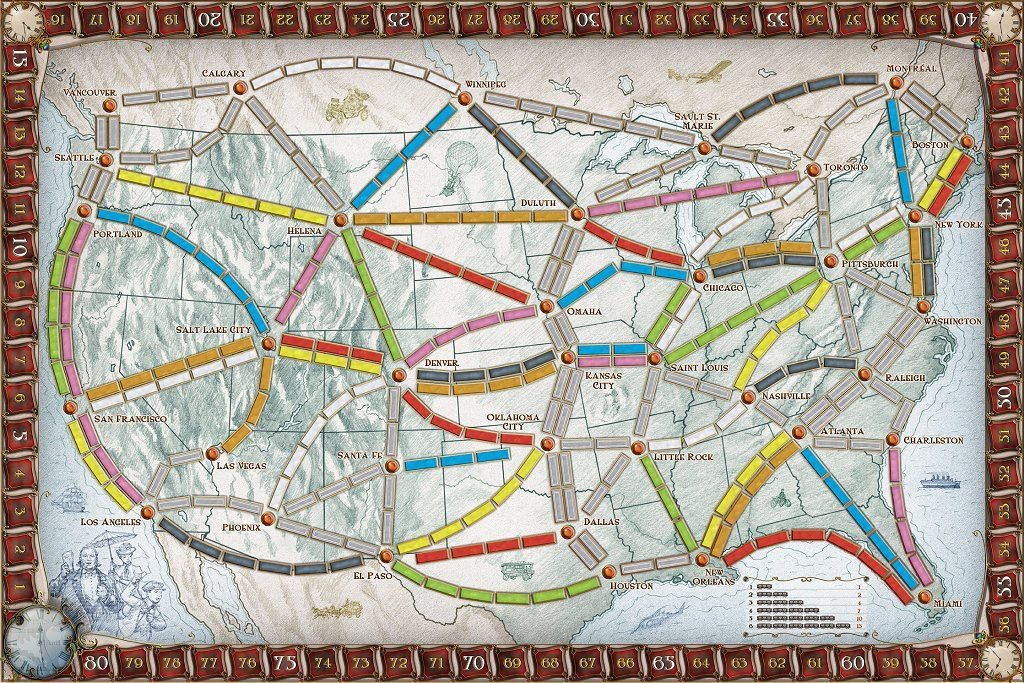
\includegraphics[scale=.2]{figures/board}
\captionof{figure}{The \textit{Ticket to Ride} U.S. board.}
\label{fig:board}
\end{figure}

Each player begins the game with four random Train Car cards.
These cards are used to buy routes.
For example, a player can use four pink Train Car cards to purchase
the route between Charleston and Miami
(at the bottom right corner of \cref{fig:board}).
At the beginning of the game 
each player also receives three Destination Ticket cards.
Two cities and a reward are specified on each Destination Ticket.
Players choose either two or three of these cards and
receive points at the end of the game based on whether
or not they completed the Destination Ticket:
if they connected the cities then they add the point reward to their
total score and
if they did not connect the cities they subtract the points from their
total score.

Players take one of three actions on their turns.
First, a player may draw two Train Car cards either
from the deck or from the five Train Car cards
kept face up on the table. 
(If a player chooses a wild card from the table
then they are limited to one Train Car card that turn.)
Second, a player may claim a route by trading in
the appropriate number and color of Train Car cards.
The gray routes on the map are purchased with
the appropriate number of any one color.
If a pair of cities have two routes between them,
no player can claim both.
Finally, a player may draw three Destination Tickets
and return up to two of them.

When one player's stock of 45 trains dips below 3 trains at the end of their turn,
every player (including that player) gets one final turn.

\subsection{Simulations}
To simulate \textit{Ticket to Ride} games, we adapted Silva et al.'s program
\cite{silva2019, witter2019}.
We maintained the vast majority of the program structure and run our simulations
on the regular U.S.A. map.
For four-player games, we include each of Silva et al.'s four agent types.
The Destination Hungry Agent chooses Destination Tickets at the beginning of the
game--with an emphasis on Destination Tickets that are geographically close--
and tries to connect them for the rest of the game.
The Route Focused Agent works toward a longer Destination Ticket then
claims longer routes.
The One Step Agent operates by choosing the most advantageous move at each
step without a long term strategy.
The Long Route Agent claims longer routes (defined as four trains or more)
with a preference for routes that help connect the player's initial Destination Tickets.
For two-player games, we simulate an equal number of all six pairings of the four
agents. 

Our modifications to the original code our primarily to simplify
our analysis and facilitate independent simulations but for one exception:
The original code allowed agents to buy the same double-route 
(double-routes are the pairs of routes that connect the same two cities)
more than once in four-player games.
In the standard rules, however, one player
cannot claim both routes to the same cities \cite{moon2004ticket}.
We adapted the \texttt{get\_free\_connections} method to ensure
agents cannot buy both double-routes.

\section{Value of Routes}
\subsection{Longer Routes are Overvalued}
The reward for owning routes substantially increases for longer routes.
From \cref{table:current_value},
we see that the trains in one- or two-train routes are worth one point
whereas the trains in the six-train routes are worth two and half points.
The ostensible reason for the increasing value per train is that
it takes much more time to collect longer routes than shorter routes.
However in \cref{sec:collecting_cards} we will show the expected 
number of turns to collect $k$ cards of a specific
color is linear in relation to $k$
(rather than polynomial like the current scoring method).

\begin{table}[h!]
\renewcommand{\arraystretch}{1.5}
\centering
\begin{tabular}{| c | c | c | c | c | c | c |}
\hline
 Route Length & 1 & 2 & 3 & 4 & 5 & 6\\
 \hline
 Points Scored & 1 & 2 & 4 & 7 & 10 & 15\\
 \hline
 Points per Train & 1 & 1 & $1.\overline{3}$ & 1.75 & 2 & 2.5\\
 \hline
\end{tabular}
\caption{The points scored for building routes by length of route
and per the number of trains.}
\label{table:current_value}
\end{table}

Longer routes are more attractive for players.
First, the reward per train is much higher.
Instead of receiving six points for six one-train routes,
a player can receive 15 points for one six-train route.
Second, players may only buy one route per turn.
It would take a player nine turns--three to collect six cards 
and six to buy six routes--to get six points from one-train routes.
In those same nine turns, a player who spends seven turns collecting
14 cards has the chance to buy two six-train routes
and then get 30 points in their last two turns.
(While it is far from guaranteed that two sets of this player's 14 cards are
six of the same color, the option to choose from five face up cards
on the table makes it more likely that the player has six of the same color.)

The longer route strategy performs even better over many turns.
In an ideal game, a player can collect 46 train cards in 23 turns
and spend eight turns (throughout or at the end) buying all six
six-train routes, one five-train route, and one four-train route.
Because the player has 46 cards, there is a very high likelihood that
they have roughly six cards of each color.
In total, they will have accumulated 107 points and ended the game in 31 turns
where each turn, on average, earns them about three and half points.
The challenge for this strategy is that, unless the player is very lucky,
the two Destination Tickets from the beginning of the game will count
against their score.
Nonetheless, the longer route strategy has remarkable potential.

\subsection{Expected Cards to Build a Route}\label{sec:collecting_cards}
In this section, we find the expected number of cards
$N_k$ we need to see in order to find the $k$ cards of a specific color
needed to build a particular route.
Our argument is that $\E[N_k]$ is better than the
current reward scheme.

Let $C$ be the set of all cards and $k$ be a fixed integer
between 1 and 6, inclusive.
Without loss of generality say we are looking
for blue cards and call this set $B$.
In order to find how long it takes to find $k$ blue cards,
think of our well-shuffled deck as
blue cards separated by non-blue cards.
For example, our deck may have the ordering
\begin{align}
    xxxbxbxxxx...xxbxxx \nonumber
\end{align}
where $x$ is a non-blue card in $C \setminus B$
and $b$ is a blue card in $B$.

Now let $N_k$ be the number of cards until
we see the $k^{th}$ blue card.
Our strategy is to write $N_k$ in terms of
indicator random variables.
Let $I_{k,x}$ be the indicator that takes value 1
if non-blue card $x$ appears before the $k^{th}$ blue card
and 0 otherwise.

The number of cards until the $k^{th}$ blue card
is certainly the number of blue cards $k$
plus the number of non-blue cards before the $k^{th}$ blue.
Written as an equation,
\begin{align}
    N_k = k + \sum_{x \in C \setminus B} I_{k,x}. \nonumber
\end{align}
We are interested in the average number of cards
so we take the expectation of $N_k$ and distribute
over addition via linearity of expectation.
Then
\begin{align} \label{eq:expected_card}
    \E[N_k] = \E[k] + |C \setminus B| \times \E[I_{k,x}].
\end{align}
Since $k$ is fixed, $\E[k]$ is simply $k$.
Since $B$ is a subset of $C$ and both sets are fixed,
$\E[|C \setminus B|]$ is $|C| - |B|$.
Thus we need only find $\E[I_{k,x}]$.

To calculate $\E[I_{k,x}]$, think of the deck as $|B| + 1$ sequences 
of non-blue cards separated by $|B|$ blue cards.
(It is possible for a sequence to be of length zero
in the case that two blue cards are adjacent to each other or
in the case that the first or last card is blue.)
Since we assume the deck is well-shuffled, the non-blue cards
are uniformly distributed across the $|B| + 1$ sequences:
it is as likely for card $x \in C \setminus B$ to be in any one sequence
as any other.

Now think of the indicator $I_{k,x}$ that card $x$ appears
before the $k^{th}$ blue in terms of which of the $|B| + 1$
sequences $x$ resides in.
When looking for only one blue card,
we see that card $x$ appears before the first blue if and only if
$x$ is in the first sequence.
Since $x$ is uniformly distributed across all $|B| + 1$ sequences,
the probability that $x$ appears before the first blue $\p(I_{1,x})$
is $1/(|B| + 1)$.
Similarly, the probability that $x$ appears before the second blue
$\p(I_{2,x})$ is $2/(|B| + 1)$.
By extension, the probability that $x$ appears before the $k^{th}$
$\p(I_{k,x})$ is $k/(|B| + 1)$.

Recall that $I_{k,x}$ takes value 1 if $x$ appears before the 
$k^{th}$ blue and 0 otherwise.
Then, conditioning on $I_{k,x}$, we write its expectation
\begin{align} \label{eq:expected_indicator}
    \E[I_{k,x}] &= 1 \times \p(I_{k,x})
    + 0 \times (1-\p(I_{k,x}) \nonumber \\
    &=\p(I_{k,x}) = \frac{k}{|B| + 1}
\end{align}
Substituting \cref{eq:expected_indicator} in \cref{eq:expected_card},
we have
\begin{align}
    \E[N_k] &= k + |C \setminus B| \times \left(\frac{k}{|B| + 1}\right)
    \nonumber \\
    &= \left(1 + \frac{|C| - |B|}{|B| + 1} \right)k. \nonumber
\end{align}
and, by plugging in the values of $|C|$ and $|B|$,
\begin{align}
    \E[N_k] &= \left(1 + \frac{110 - 12}{12 + 1} \right)k \nonumber \\
    &= \frac{111}{13}k. \nonumber
\end{align}
While the value $111/13$ has no obvious units or interpretation,
we have learned that $\E[N_k]$ is proportional to $k$.
That is, $\E[N_k] = \alpha k$ for some $\alpha$.
If we use $\E[N_k]$ as the points scored by buying a route of length
$k$, the value of $\alpha$ will matter relative to the points from
connecting Destination Tickets and the longest path.
In the next section, we use Silva et al.'s simulation
to find the $\alpha$ for which their longest route
agent wins roughly as often as their other agents.

\subsection{Optimal Route Value via Simulations}

\newpage
\section{Destination Tickets}

\subsection{Winning}
An obvious strategy in \textit{Ticket to Ride} is to collect
Destination Tickets and buy routes to connect them.
We investigate the effect of collecting Destination Tickets
on winning the game.
We simulate 10,000 two-player and 10,000 four-player games.
For each Destination Ticket, we calculate the proportion of 
games that the player holding the Destination Ticket won.
Our results appear in \cref{fig:tickets}.
(For example, players in two-player games with Phoenix to Portland
won almost exactly half of their games.)

\begin{figure}[h]
\centering
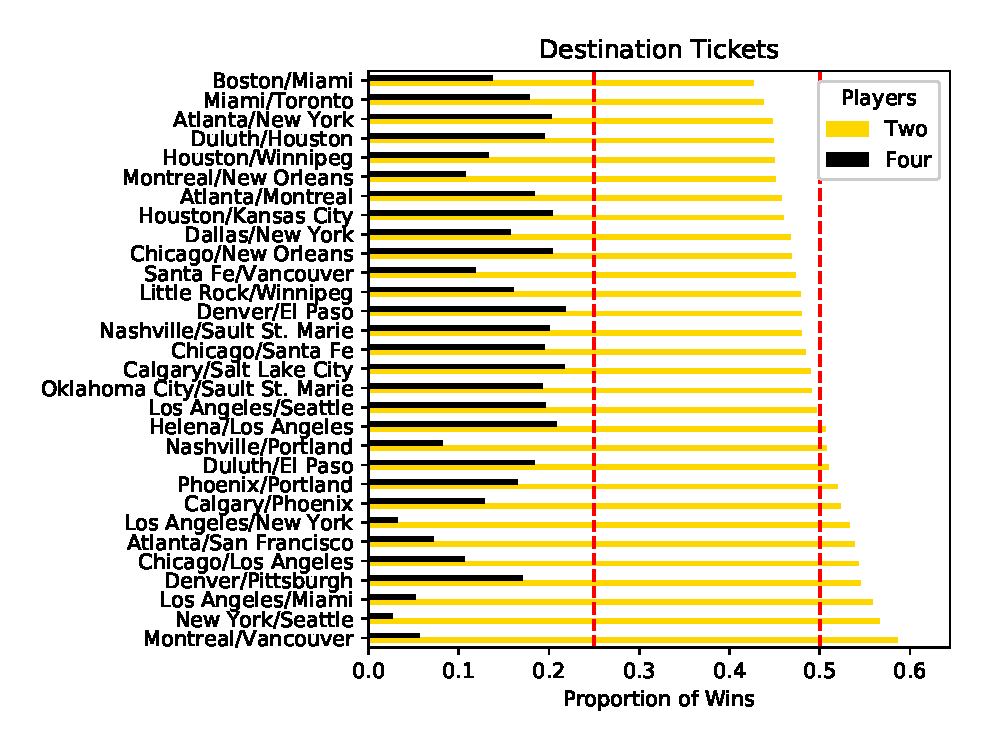
\includegraphics[scale=.6]{figures/destination_tickets}
\caption{For each Destination Ticket,
the proportion of two-player and four-player games that 
the player with the Destination Ticket won.
The vertical red lines at $1/4$ and $1/2$ represent
the expected proportion of games players would win
if Destination Tickets had no effect.}
\label{fig:tickets}
\end{figure}

The vertical red lines at .25 and .5 indicate
the expected proportion of wins if Destination Tickets
had no effect on winning: players in two-player games
would win half the time and players in four-player games
would win a quarter of the time.

In two-player games, there are 13 Destination Tickets 
that win more than the expected $50\%$ of games.
In four-player games, there are only eight Destination Tickets
that clearly win more than the expected $25\%$ of games plus
another four on the borderline.
That is, out of the 30 Destination Tickets, roughly a third
in both two- and four-player games win more than expected.
The implication is that a randomly chosen Destination 
Ticket is not advantageous.
However, a subset of Destination Tickets--approximately the same
set for both two- and four-player games--wins more often than expected.
The ones that win the most are Montreal to Vancouver,
New York to Seattle, and Chicago to Los Angeles.

An inspection of \cref{fig:board} shows that the paths between 
these three Destination Tickets are some of the longest on the board 
and include routes with the most trains.
However, to gain a better understanding of what makes some
Destination Tickets more advantageous than others,
we investigate their characteristics
that most closely correlate with winning.
We begin in the next subsection by developing a measure
of the difficulty of connecting one city to another.

\subsection{Effective Resistance}
The \textit{Ticket to Ride} board can mathematically
be interpreted as a graph where cities represent
nodes and routes represent edges.
Thus, to analyze the difficulty of connecting a
pair of cities we can frame the problem in graph theoretic language.
One of the most powerful and natural measures
between two nodes on a graph is effective resistance
\cite{ellens2011effective}.
Imagine that the \textit{Ticket to Ride} board was
a large electrical circuit with a unit current
entering at city $a$ and leaving at city $b$.
Effective resistance indicates
how much work a current needs to exert
to get from $a$ to $b$.
In general, the number of paths and length of routes 
determine the effective resistance:
two cities with fewer paths and longer routes
have a higher effective resistance between them
than two cities with many paths and shorter routes.
We calculate the effective resistance for each 
Destination Ticket in order to gain insight
into what makes some more advantageous than others.

On a small graph, effective resistance can be calculated
by repeatedly applying the following rules:
Consider two edges with resistances $r_1$ and $r_0$.
If the two edges are in series (edge 1 connects node $i$ to $j$
and edge 2 connects node $j$ to $k$), then the resistance between
$i$ and $k$ is $r_1 + r_2$.
If the two edges are in parallel (both edge 1 and edge 2 connect
node $i$ to $j$), then the resistance between $i$ and $j$
is $(1/r_1 + 1/r_2)^{-1}$.

On a large graph like the \textit{Ticket to Ride} board, 
we need a more robust strategy.
We use two separate algorithms to find the effective resistance
of Destination Tickets
\cite{ellens2011effective, wu2004theory}.
Both algorithms calculate the effective resistance by finding 
the eigenvalues of the Laplacian matrix for a given graph.
(The Laplacian is the degree matrix $D$ minus the adjacency
matrix $A$ where $D_{i,i}$ is the weighted degree of node $i$
and $A_{i,j}$ is the resistance of the edges between nodes
$i$ and $j$.)

We let the weight between two cities be the number
of trains of the route connecting them.
In the case that there are two routes between cities,
we let the weight be $(1/r + 1/r)^{-1}=r/2$ where
$r$ is the number of trains of each route.

In the next subsection, we calculate the effective
resistance of all Destination Tickets as a tool
to find what most closely correlates with winning.

\begin{figure}[h]
    \centering
    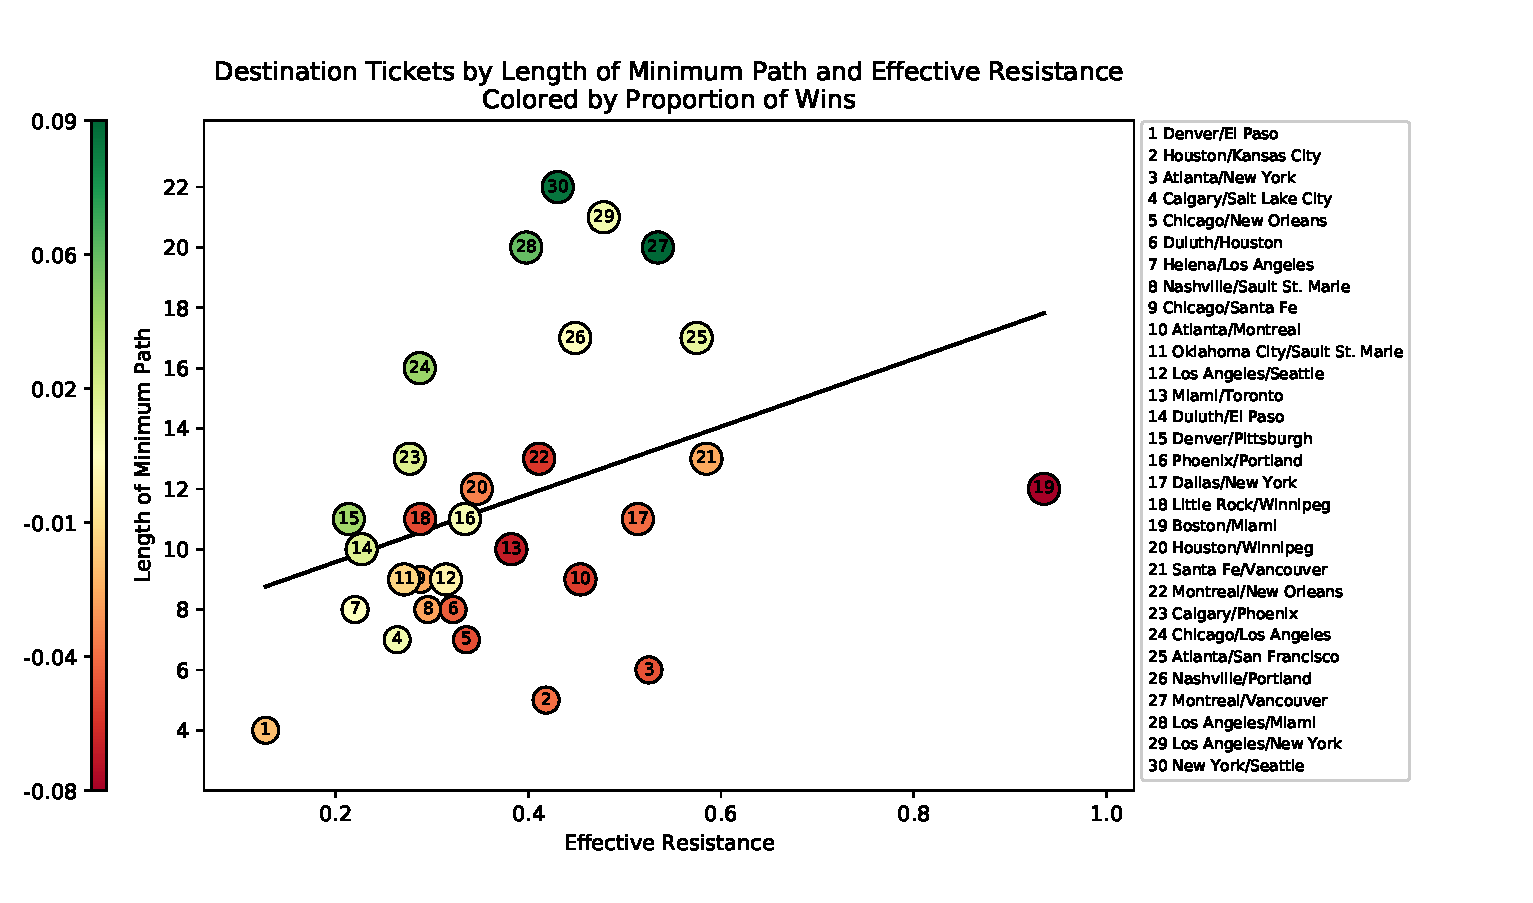
\includegraphics[scale=.6]{figures/resistance_aggregate}
    \caption{Destination Tickets plotted by their effective
    resistance and minimum path length and colored
    by overall proportion of wins.
    The line of best fit gives an approximation of the
    Destination Tickets that have a higher reward per difficulty
    (above the line).
    Note: the $9^{th}$ Destination Ticket 
    is obscured by the $11^{th}$.}
    \label{fig:resistance}
\end{figure}

\subsection{Winning \& Effective Resistance}

In \cref{fig:resistance},
Destination Tickets are plotted by their effective resistance
and minimum path length.
Recall that the reward for connecting a Destination Ticket
is the length of the shortest path between its two cities.
Since effective resistance measures the difficulty of
connecting the two cities, the line of best fit in \cref{fig:resistance}
indicates reward per difficulty.
The Destination Tickets above the line of best fit are
a "good" deal relative to the rest of the Destination Tickets
whereas those below the line of best fit are a "bad" deal.

The proportion of wins (also dubbed overall wins
in \cref{fig:correlation_table} and \cref{fig:correlation_figures})
is the difference from the expected proportion of wins
across two- and four-player games.
For example, a Destination Ticket with a value of .05 indicates
that players with that destination Ticket 
win on average $30\%$ of four-player games
(rather than the expected $25\%$) and $55\%$ of 
two-player games (rather than the expected $50\%$).

We use the proportion of wins as a proxy for the desirability
of Destination Tickets and attempt to interpret what variables
increase player wins from \cref{fig:resistance}.
It appears that Destination Tickets with longer minimum paths win
more as well as Destination Tickets with a smaller effective resistance.
But the correlation between either variable and the proportion
of wins is not clear-cut.

\cref{fig:correlation_table} shows the Pearson correlation statistic
between wins and various (possibly) related variables.
The path length and resistance are the y- and x-axes of 
\cref{fig:resistance}.
The residual is the difference between the predicted
path length (line of best fit) and the actual path length
in \cref{fig:resistance}.
The results indicate that path length is well correlated with wins,
resistance is not correlated with wins, and residual is very
well correlated with wins.
\cref{fig:correlation_figures} shows the data points and
their relationship to wins summarized in
in the last column of \cref{fig:correlation_table}.

\begin{figure}[h]
    \centering
    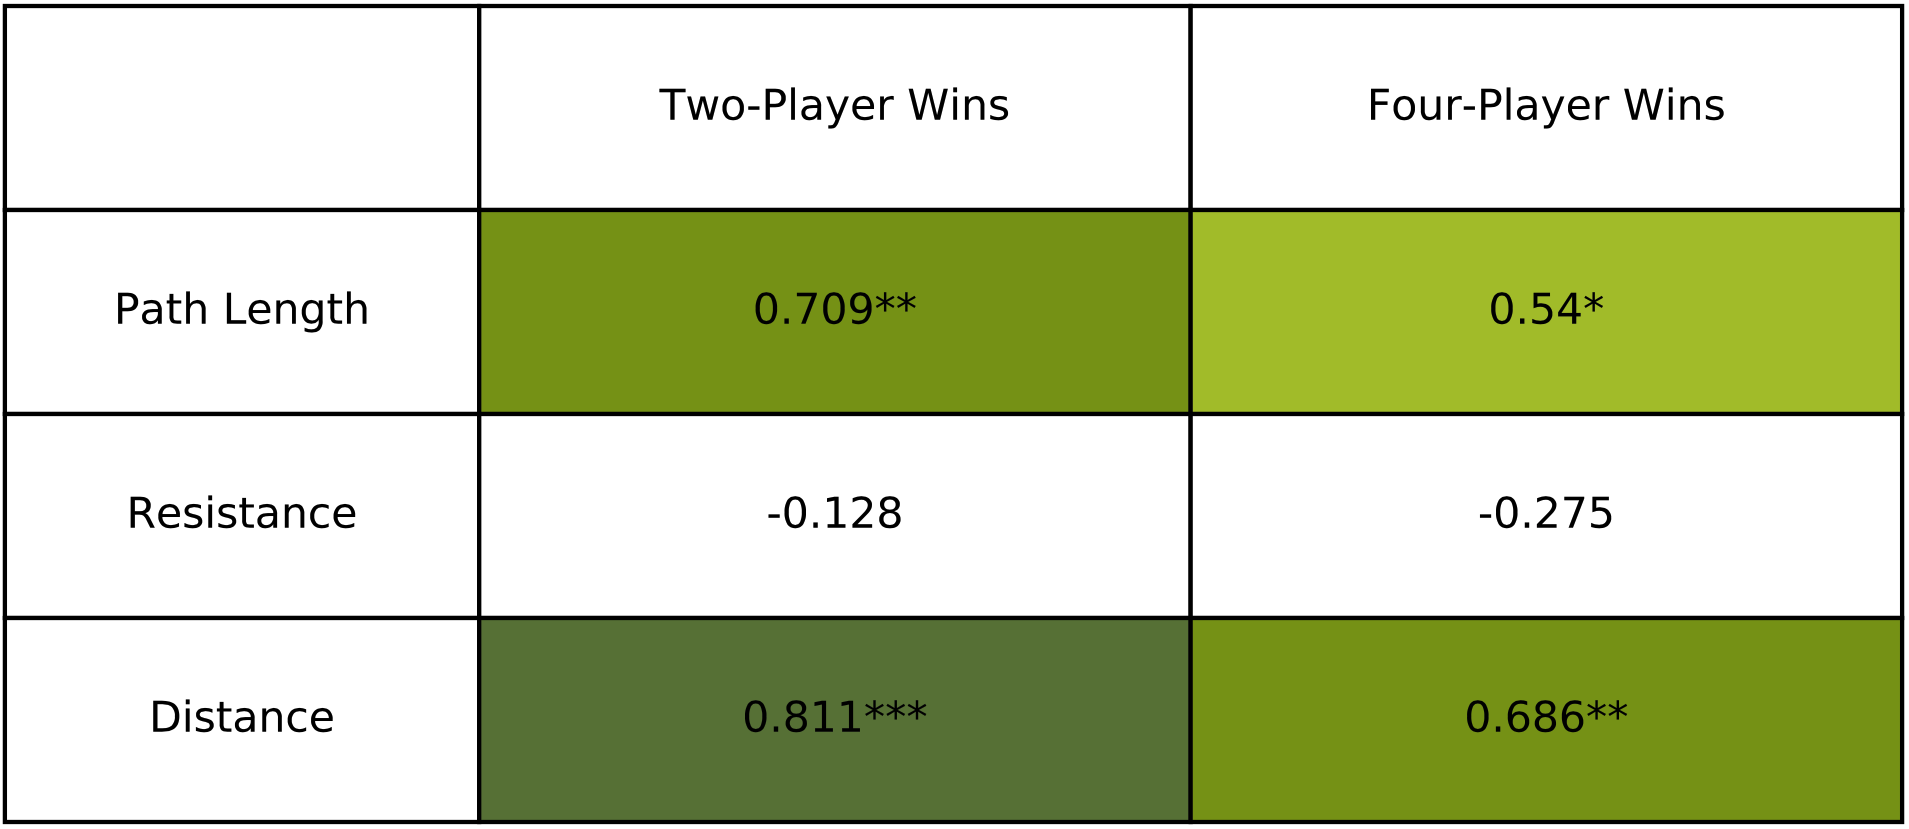
\includegraphics[scale=.12]{figures/pearsons_table.png}
    \caption{The Pearson correlation statistic between
    the win proportion of Destination Tickets
    and measures of difficulty.
    A single asterisk (in light green) indicates a p-value
    below 1E-2. Double asterisks (in green) indicate a
    p-value below 1E-4. Triple asterisks (in dark green)
    indicate a p-value below 1E-6.}
    \label{fig:correlation_table}
\end{figure}

\begin{figure}[H]
    \centering
    \begin{subfigure}[t]{0.36\textwidth}
        \centering
        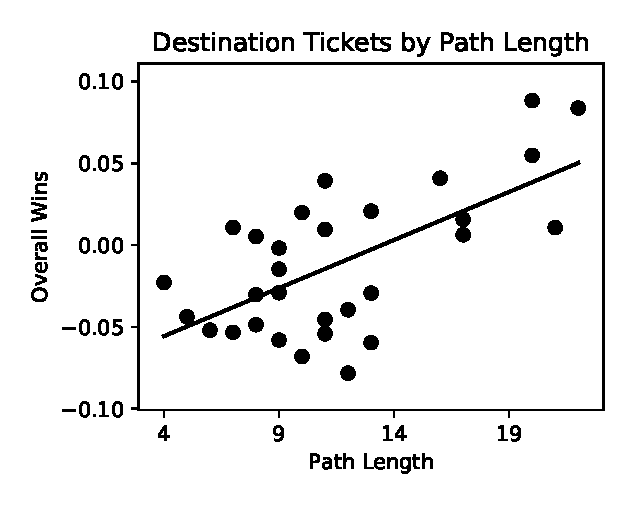
\includegraphics[height=1.7in]{figures/correlation0}
    \end{subfigure}%
    ~ 
    \begin{subfigure}[t]{0.36\textwidth}
        \centering
        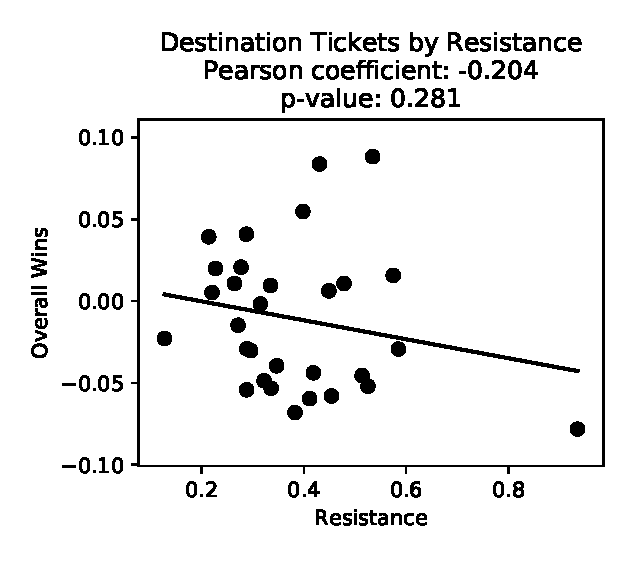
\includegraphics[height=1.7in]{figures/correlation1}
    \end{subfigure}%
    ~ 
    \begin{subfigure}[t]{0.36\textwidth}
        \centering
        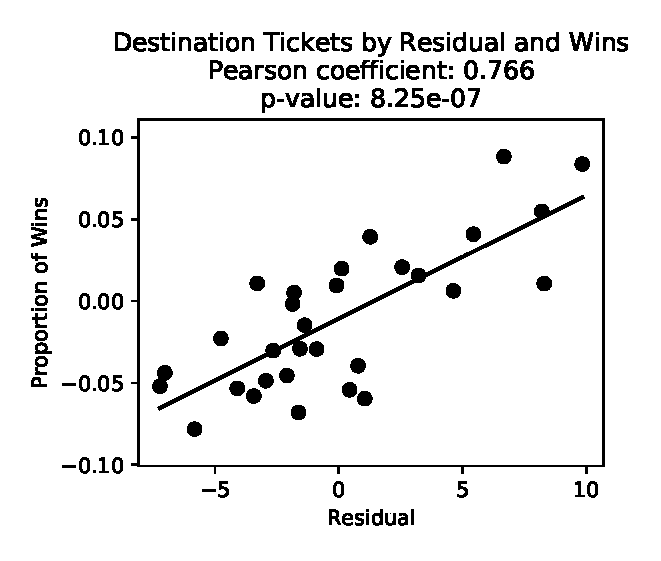
\includegraphics[height=1.7in]{figures/correlation2}
    \end{subfigure}%
    \caption{Destination Tickets by the
    difference between the expected proportion of wins
    and (possibly) related variables.
    The last column of \cref{fig:correlation_figures}
    indicates how closely the lines of best fit
    model Destination Tickets.}
    \label{fig:correlation_figures}
\end{figure}

While path length is a good predictor 
of which Destination Tickets win, 
the residual from the model built from effective resistance
is even better (\cref{fig:correlation_table} and
\cref{fig:correlation_figures}).
\cref{fig:rankings} shows the change in rankings
between path length and residual.

Even though it is easier to compare path length when choosing
between Destination Tickets in real time,
learning the most advantageous Destination Tickets may be worthwhile:
as a general rule, Destination Tickets with a minimum path
longer than 15 trains or those with small effective resistance
(many short paths) outperform their counterparts.

Referring to \cref{fig:resistance}, 
we provide several explanations for why Destination Tickets 
win more than expected.
The Destination Tickets with more than 15 trains 
enjoy high rewards and middle-of-the-pack 
resistances.
In addition, they benefit from the advantages of longer 
routes discussed in \cref{sec:overvalued}.
The remaining Destination Tickets--below or slightly 
above the line of best fit--seem to be more affected
by resistance: the higher the resistance, the
lower the proportion of wins.
Perhaps because the resistance between these pairs of cities
is roughly comparable, Destination Tickets that 
can be connected more easily help players more.

\begin{figure}[H]
    \centering
    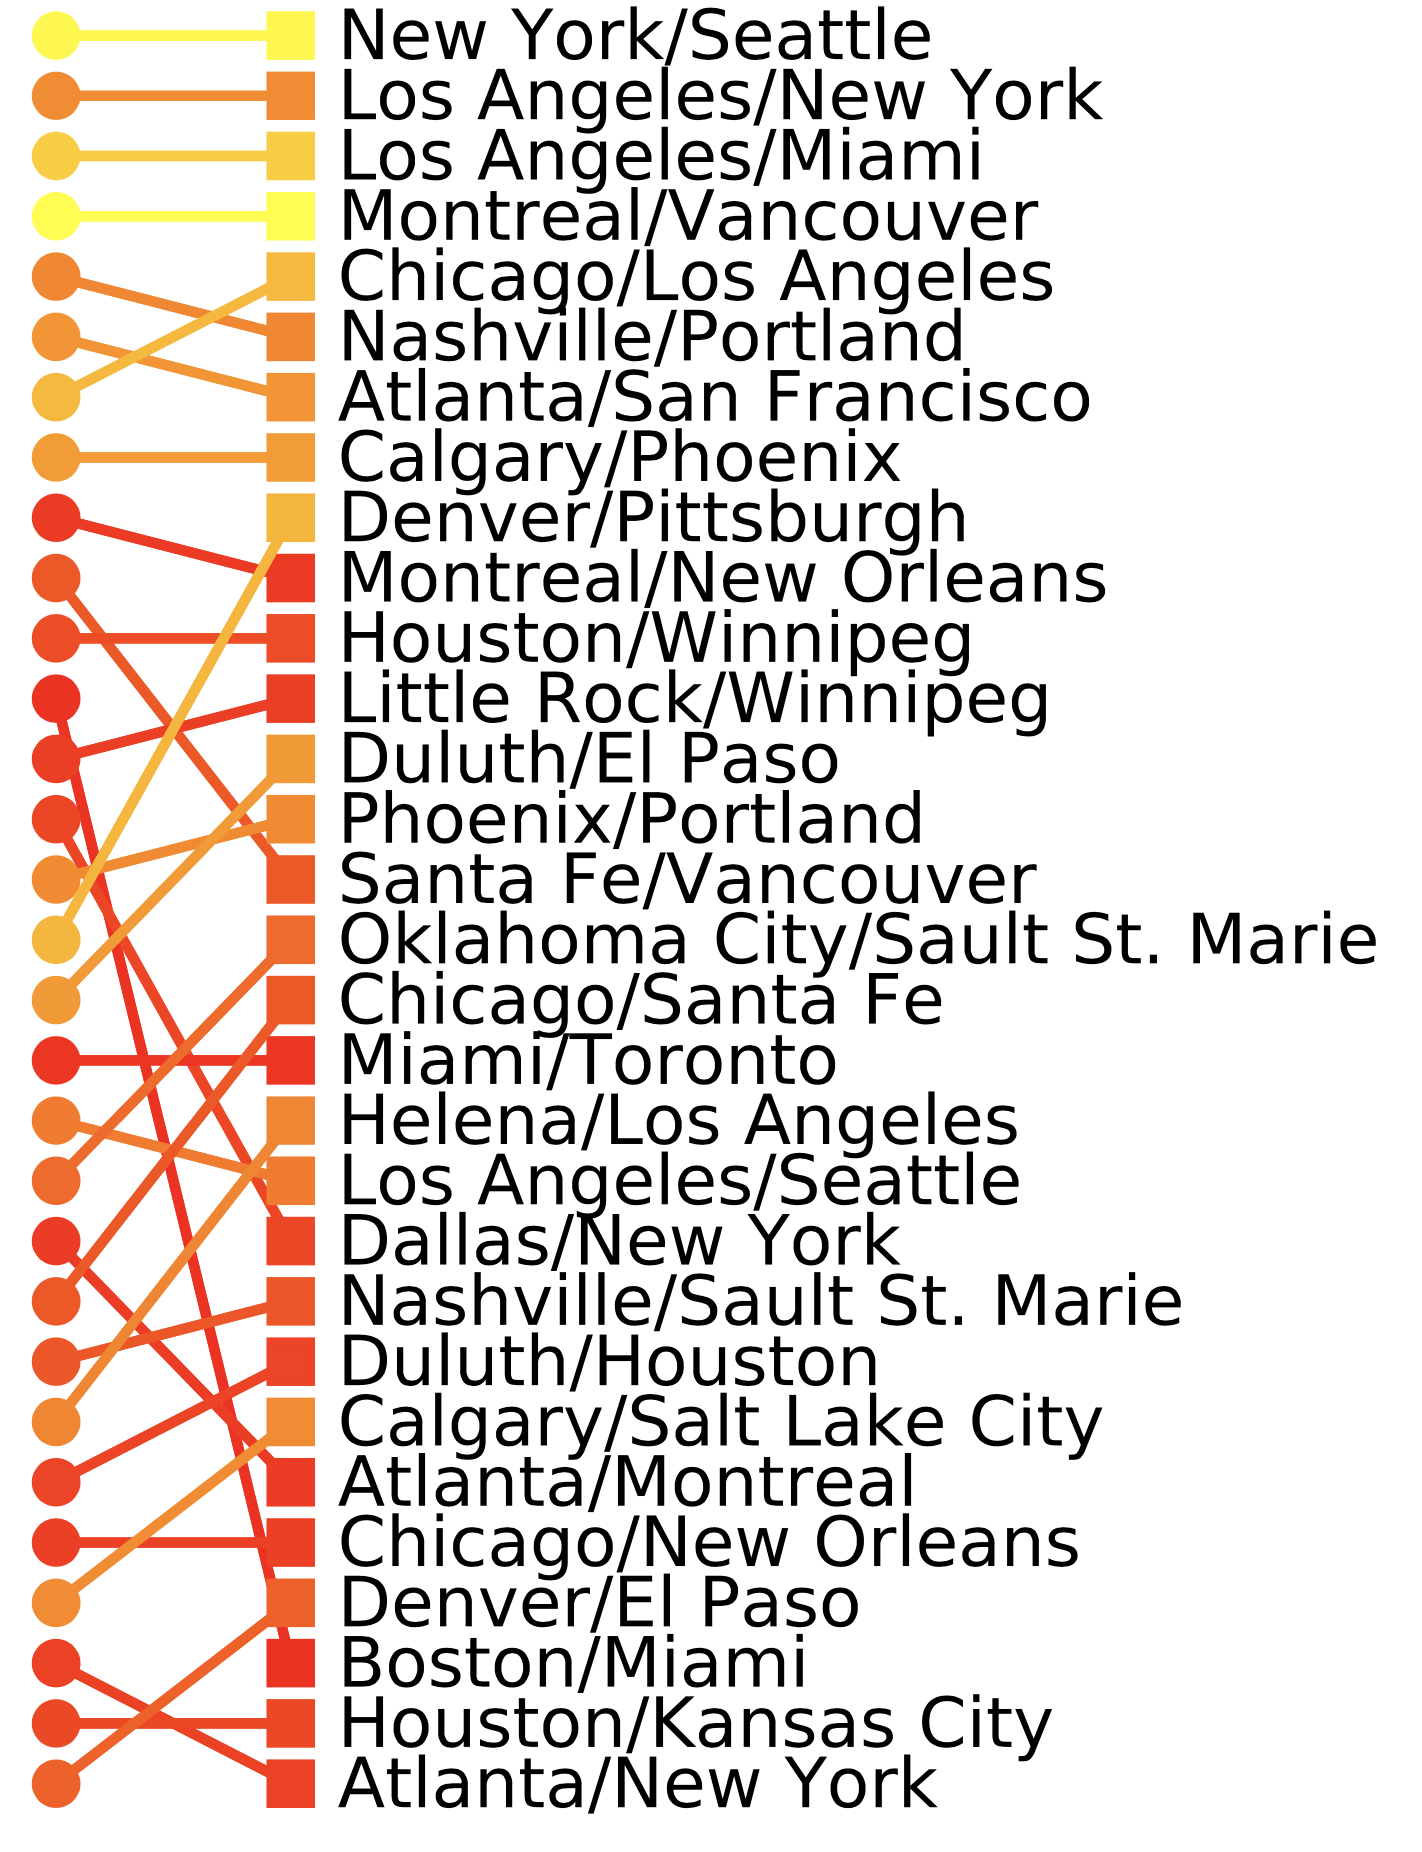
\includegraphics[scale=.25]{figures/rankings.png}
    \caption{Destination Tickets ordered by path length
    in the left column (circles) and by residual
    in the right column (squares). The color
    corresponds to the proportion of overall wins (scale
    from \cref{fig:resistance}).
    Lines indicate the change in rank between
    the two orderings.}
    \label{fig:rankings}
\end{figure}


\section{Routes \& Betweenness Centrality}

\begin{figure*}[!ht]
\centering
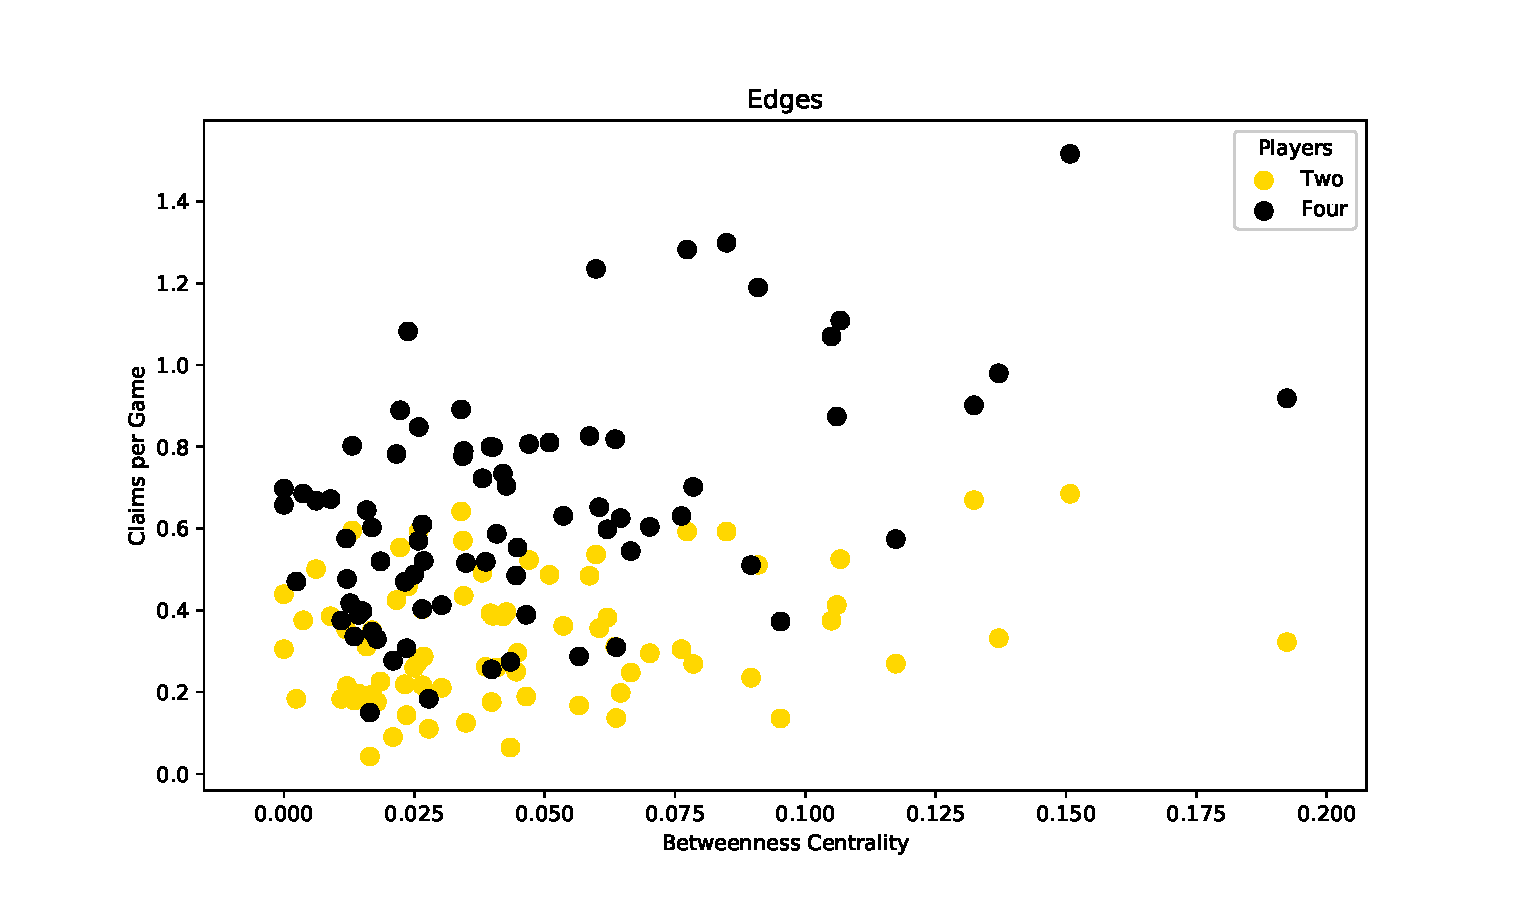
\includegraphics[scale=.7]{figures/centrality_betweenness}
\caption{The 30 most frequently routes claimed
per game.
(Some cities have two routes between them so it is
possible for a route to be claimed more than once per game.)}
\label{fig:routes}
\end{figure*}
 
\bibliographystyle{abbrv}
\bibliography{main}

\end{multicols}{2}
\end{document}
